\documentclass[11pt,a4paper]{article}
\usepackage{fontspec}
\usepackage{polyglossia}
\setmainlanguage{ukrainian}
\setotherlanguage{english}
\setmainfont{cmunrm.otf}[Path=fonts/,BoldFont=cmunbx.otf,ItalicFont=cmunti.otf,BoldItalicFont=cmunbi.otf]
\setsansfont{cmunss.otf}[Path=fonts/,BoldFont=cmunsx.otf,ItalicFont=cmunsi.otf,BoldItalicFont=cmunso.otf]
\setmonofont{cmuntt.otf}[Path=fonts/,ItalicFont=cmunit.otf]
\newfontfamily\cyrillicfont{cmunrm.otf}[Path=fonts/,BoldFont=cmunbx.otf,ItalicFont=cmunti.otf,BoldItalicFont=cmunbi.otf,Script=Cyrillic]
\newfontfamily\cyrillicfontsf{cmunss.otf}[Path=fonts/,BoldFont=cmunsx.otf,ItalicFont=cmunsi.otf,BoldItalicFont=cmunso.otf,Script=Cyrillic]
\newfontfamily\cyrillicfonttt{cmuntt.otf}[Path=fonts/,ItalicFont=cmunit.otf,Script=Cyrillic]
\usepackage[a4paper,margin=25mm]{geometry}
\usepackage{microtype}
\usepackage{booktabs,longtable,tabularx,array,multirow}
\usepackage{graphicx}
\graphicspath{{figures/}}
\usepackage{caption}
\captionsetup{font=small,labelfont=bf,labelsep=colon,justification=justified,singlelinecheck=false}
\captionsetup[table]{position=top}
\usepackage{enumitem}
\usepackage{amsmath}
\usepackage{float}
\usepackage[section]{placeins}
\usepackage[numbers,sort&compress]{natbib}
\usepackage{xurl}
\usepackage{hyperref}
\urlstyle{same}
\hypersetup{hidelinks,pdfencoding=auto,unicode=true,pdftitle={Від локального інциденту до інформаційної хвилі},pdfauthor={Олександр Пилипенко}}
\emergencystretch=2em
\setlist{nosep,leftmargin=1.5em}
\renewcommand{\arraystretch}{1.12}
\renewcommand{\bibfont}{\small}
\setlength{\bibsep}{2pt}
\begin{document}
\title{\LARGE Від локального інциденту до інформаційної хвилі: дослідження цифрових слідів у Петропавлівській Борщагівці, Україна (2–9 листопада 2026 року)}
\author{Олександр Пилипенко\\[0.4em]
\small Незалежний дослідник у сфері штучного інтелекту та машинного навчання\\[0.2em]
\small Аспірант Державного торговельно-економічного університету, Київ, Україна\\[0.2em]
\small ORCID: 0009-0004-9610-9242\\[0.2em]
\small \texttt{O.Pylypenko@knute.edu.ua}}
\date{2026-11-09}
\maketitle

\begin{abstract}
\noindent У статті досліджено, що можна встановити з обмеженого набору публічних цифрових слідів про інформаційну хвилю довкола інциденту 2 листопада 2026 року в Петропавлівській Борщагівці. Поєднано цільову панель Telegram, відібрані гілки коментарів, надані посилання TikTok, метадані й субтитри YouTube, публічні заяви, куровану матрицю «твердження—доказ», умовні перестановочні тести та бенчмарк транскрипції 18 кліпів. Базовий корпус містить 23\,350 дописів, зокрема 1\,408 релевантних записів у 159 із 241 моніторингового ідентифікатора. У матриці 25 тверджень 19 підтримано в межах визначеного обсягу доказів, а для шести доказів недостатньо; два центральні твердження про фізичні обставини лишаються невстановленими. Окремі статистики повторів і часу перевищили всі 9\,999 симуляцій визначених умовних нульових моделей, що вказує на нетипову синхронізацію, але не встановлює її організатора чи мотив. Мікро-WER у бенчмарку мовлення становив 44,58\%; лише 10 із 18 кліпів пройшли перевірку безпечності цитування. Відео пожежі з TikTok візуально збігається з наданою копією, але його місце зйомки та зв'язок із попереднім зіткненням не підтверджено. Стаття характеризує спостережувані записи, а не громадську думку, охоплення, переконання чи остаточну фізичну хронологію.
\end{abstract}

\noindent\textbf{Ключові слова:} обчислювальна соціальна наука; кризова інформатика; цифрові сліди; Telegram; перевірка тверджень; сигнали координації; невизначеність вимірювання; Україна

\noindent\textbf{Обсяг доказів.} Збір даних із платформ був цільовим і неповним. Кількості описують лише задокументовані зрізи; вони не є оцінками для всієї платформи, виміром громадської думки чи незалежною перевіркою кожного фізичного твердження.

\section{Вступ}

Соціальні платформи роблять локальні події видимими через швидкі й фрагментовані сліди: короткі дописи, репости, коментарі, відеофрагменти й офіційні повідомлення. Ці матеріали допомагають документувати, коли з'являлися публічні твердження та як вони поширювалися. Водночас вони створюють складну проблему вимірювання. Багаторазово повторене повідомлення може походити від одного свідчення; часову позначку допису не можна автоматично вважати часом показаної події; а заява установи є доказом її позиції, але не обов'язково незалежним підтвердженням кожного фізичного факту. Розрізнення інформаційного поширення та перевірки самої події є центральним для кризової інформатики й досліджень дезінформації \citep{lazer2018science,vosoughi2018spread,han2019rumour}.

У статті описано обмежене дослідження інформаційної хвилі довкола подій у Петропавлівській Борщагівці Київської області 2 листопада 2026 року та подальших обговорень до 9 листопада. Кейс важливий для аналізу, бо в ньому перетинаються кілька типів невизначеності: ранні повідомлення про людей у будівлі; офіційні заперечення та незавершені перевірки; суперечливі описи травм і умов; мобілізація та пошкодження майна; а також пізніше відео складської пожежі з підписом назви сусіднього населеного пункту. Питання дослідження не в тому, чи має одна платформа або установа повну картину. Ми з'ясовуємо, які висновки можна відповідально зробити з неповного й нерівномірно доступного цифрового матеріалу.

Стаття має три практичні внески. По-перше, інформаційне середовище описано через окремі знімки й знаменники, а не одним числом, що нібито репрезентує всю платформу. По-друге, повторювані тексти аналізуються через аудит точних пар і умовні перестановочні тести, із чітким відокремленням нетипових координаційних ознак від атрибуції. По-третє, показано підхід до визначення обсягу доказу, за якого твердження може бути підтверджене як факт висловлювання, процесуальний крок або обмежене спостереження, але це саме по собі не встановлює відповідний фізичний факт. Такий підхід узгоджується з методологічними застереженнями щодо упереджень збору, доступу й платформних механізмів, а також ризиків хибнопозитивної автоматичної класифікації ботів \citep{olteanu2019social,rauchfleisch2020false,vicente2023sampling}.

\section{Визначення кейсу та дослідницькі питання}

Об'єкт дослідження — публічне зіткнення біля будівлі в Петропавлівській Борщагівці 2 листопада. Інформаційний епізод охоплює дописи й коментарі про будівлю, перебування та поводження з військовослужбовцями, реакцію поліції та інших установ, твердження про незаконне утримання чи загибель, а також пізніші наративи, які пов'язують із попереднім зіткненням окрему складську пожежу. Часові вікна різняться за джерелами: основний період дописів Telegram завершується 5 листопада о 12:10:13 за Києвом; знімки коментарів та інших платформ збирали пізніше; основний звіт зафіксовано 9 листопада. Це різні часові межі, їх не можна механічно звести до однієї.

Дослідницькі питання:
\begin{enumerate}
\item Який обсяг і часовий профіль релевантних дописів спостерігається в моніторинговій панелі Telegram і які частини платформи залишаються поза спостереженням?
\item Які публічні твердження можна пов'язати з конкретними джерелами та фрагментами доказів, а які лишаються спірними або недостатньо підтвердженими?
\item Чи відрізняються повтори дописів і коментарів від очікуваного розподілу за визначеними умовними нульовими моделями?
\item Що можна встановити про міжплатформну плутанину навколо відео пожежі, а що лишається неперевіреним щодо самого відео?
\item Які методологічні обмеження виникають під час автоматизованої реконструкції реального інциденту за неповними публічними слідами?
\end{enumerate}

Оцінюваний об'єкт — розподіл записів у зібраних і чітко визначених знімках. Це не розподіл переконань усіх користувачів платформи, мешканців України чи населення загалом. Коментатори є самовідібраною групою, видимість повідомлень залежить від ранжування та модерації, а метод збору не створює ймовірнісної вибірки \citep{olteanu2019social,vicente2023sampling,pfeffer2023sample}.

\section{Інституційний контекст і межі доказів}

Поліція Київської області оприлюднила заяву 2 листопада о 17:27. У ній зазначено, що поліцію викликали працівники приватної швидкої допомоги, біля приватного будинку перебували військовослужбовці Національної гвардії та місцеві жителі, а повідомлення про незаконне утримання та загиблого не відповідають дійсності, водночас обставини ще з'ясовувалися \citep{npu2026statement}. Пізніше ввечері МВС оголосило службову перевірку. 3 листопада ДБР повідомило про кримінальне провадження щодо подій і обставин перебування військовослужбовців у приміщенні \citep{dbr2026proceeding}. На брифінгу 3 листопада командувач Нацгвардії, як передало МВС, сказав, що в будівлі перебували 26 військовослужбовців, четверо з яких повернулися після самовільного залишення частини, а інші чекали на базову підготовку; умови він назвав належними \citep{mvs2026briefing}.

Це важливі заяви джерел. Вони засвідчують, що саме й коли публічно повідомили відповідні установи. Самі по собі вони не є завершеною незалежною інспекцією, медичною документацією, повним переписом осіб або судовим висновком. У корпусі проєкту не було завершеного публічного звіту перевірки, який незалежно розв'язував би всі суперечки щодо фізичних обставин. 5 листопада Національна поліція повідомила, що встановила 130 осіб у зв'язку із заворушеннями; встановлення особи та повідомлення про підозру є процесуальними етапами, а не обвинувальними вироками \citep{npu2026identified}. Тому дослідження не приписує конкретним людям вину чи приховані мотиви.

Пізніша складська пожежа є окремим, хоча пов'язаним інформаційним епізодом. Інтерфакс-Україна 5 листопада о 00:05 повідомив, що після атаки загорівся склад у Бучанському районі, посилаючись на голову Київської обласної військової адміністрації; агентство зазначало, що конкретне розташування в Софіївській Борщагівці на той момент офіційно не було підтверджене \citep{interfax2026fire}. Допис Борщагівської сільської ради близько 00:17 назвав Софіївську Борщагівку та складські приміщення \citep{village2026fire}. Оригінальні тексти дописів у репозиторії не збережені; цей ланцюг задокументовано аудитом джерел, а не повною локальною копією. Жодне з цих джерел не геолокує ролик TikTok, наданий дослідницькому проєкту.

\section{Дані та методи}

\subsection{Джерела даних і вибірка}

\subsubsection{Публікації Telegram}

Базова вибірка містить 23\,350 зібраних дописів і 1\,408 релевантних дописів у 159 каналах із 241 моніторингового ідентифікатора каналу. Основне вікно триває від 2 листопада 00:00 до 5 листопада 12:10:13 за Києвом, початок включений, кінець виключений. Релевантні дописи визначено в цільовій панелі моніторингу, сформованій із початкового списку каналів і розширеної за видимими пересиланнями та посиланнями. Це не випадкова вибірка Telegram; приватні й недоступні простори до неї не входять. У 49 із 1 408 релевантних записів не було лічильника переглядів, а 459 не містили тексту; покриття тому неоднорідне.

Окремий розширений знімок налічує 1\,438 релевантних дописів у 158 каналах і використовувався у пізнішому автономному аналізі. Його квитанція збору й обробки датується 8 листопада. Це не виправлення, яке можна непомітно злити з базовим корпусом: у кожному результаті статті вказується конкретний знімок. Сума поточних лічильників розширеного знімка — 119\,515\,745, базового — 115\,931\,014. Це суми лічильників, зафіксованих під час збору. Перегляди можуть повторюватися, аудиторії перетинаються, тому жодна із сум не вимірює кількість унікальних людей, фактичну експозицію на момент публікації чи переконання.

\begin{table}[!t]
\centering
\small
\caption{Зібрані набори даних і зміст їхніх знаменників.}
\begin{tabularx}{\textwidth}{>{\raggedright\arraybackslash}p{0.22\textwidth}>{\raggedright\arraybackslash}p{0.23\textwidth}>{\raggedright\arraybackslash}X}
\toprule
\bfseries Набір & \bfseries Спостережений обсяг & \bfseries Інтерпретація та обмеження \\
\midrule
Базові дописи Telegram & 23\,350 усіх; 1\,408 релевантних; 159/241 каналів & Цільова панель, основне вікно 2–5 листопада; не весь Telegram і не ймовірнісна вибірка. \\
Розширений знімок Telegram & 1\,438 релевантних; 158 каналів & Окремий знімок 8 листопада для окремих автоматизованих підсумків; має власний знаменник. \\
Коментарі Telegram & 39\,598 записів; 533 відібрані гілки; 12\,797 псевдонімізованих авторів із доступними ID & Гілки відібрані цільово, зокрема за активністю; повнота всередині гілки не робить набір репрезентативним. \\
Посилання TikTok від користувача & 42 URL: 21 відео і 21 фотодопис & Метадані отримано для 21 відео; зображення фотодописів не зібрано. Не пошукова рамка всієї платформи. \\
Обговорення відео пожежі в TikTok & 883 коментарі до цільового відео; 724 псевдонімізовані автори & 69 кандидатів вручну переглянуто; решту 814 не кодували, тому підвибірка не оцінює поширеність позицій. \\
YouTube & 617 кандидатних записів метаданих; 444 лексичні збіги; 25\,933 коментарі до 30 найпопулярніших відео & Пошук кандидатів і лексична вибірка; повний зміст відео не переглянуто. \\
Instagram, X, Threads, Facebook & Неповний або недоступний збір & Відсутність даних не означає відсутності обговорення. \\
\bottomrule
\end{tabularx}
\caption*{\small\textit{Примітка.} Кількості стосуються різних цільових зрізів платформ і не є безпосередньо порівнюваними оцінками повного обсягу активності.}
\end{table}

Корпус коментарів Telegram містить 39\,598 записів, із них 39\,459 мають доступний ідентифікатор автора, а 139 — ні. Проєкт псевдонімізував 12\,797 ідентифікаторів. 533 гілки обирали для дослідження, зокрема за активністю; повний збір усередині гілки не перетворює сукупність гілок на репрезентативну. Медіанний внесок автора — один коментар, але невелика кількість акаунтів пише значно частіше. Один відсоток найактивніших авторів створив 18,9\% коментарів доступного корпусу. Зважування за коментарями й зважування за авторами відповідають на різні питання.

\subsubsection{Інші платформи й медіаматеріали}

У межах дослідження зібрано 42 посилання TikTok, надані користувачем: 21 відеодопис і 21 фотодопис. Метадані отримано для 21 відео, зокрема підписи для 20. Фотоматеріали не завантажували. Для окремого TikTok-ролика з пожежею знімок містив 883 коментарі: 345 верхнього рівня та 538 відповідей від 724 псевдонімізованих авторів. Один анотатор вручну переглянув 69 відібраних за правилами коментарів; їх добирали для оцінювання кандидатних інтерпретацій, а не для оцінки частки всіх коментаторів, які поділяли певну думку.

Пошук YouTube дав 617 кандидатних записів метаданих. Лексичне правило звузило вибірку до 444 відео на 190 каналах із 34,6 млн поточних переглядів і 44 записами прямих ефірів. Звіт окремо описує 25\,933 коментарі до 30 найпопулярніших відео. Інша цільова вибірка субтитрів містила 49 непорожніх файлів транскрипції та 56 контекстних фрагментів із 49 відео. Повністю весь відеокорпус не переглядався. Збір Instagram обмежили вхід і ліміти запитів; доступ до X не спрацював через відсутність API-кредитів; Threads і Facebook не збирали. Отже, докази дуже нерівномірно покривають платформи.

Технічний медіареєстр кейсу містив 607 унікальних Telegram-відео, що пройшли повне декодування, із загальною тривалістю аудіо близько 14,2 години. Технічне декодування засвідчує, що файл вдалося прочитати; воно не підтверджує дату чи місце зйомки, належність до події, автентичність або правильність підпису. Окремий бенчмарк транскрипції мовлення охопив 18 кліпів із акустичними еталонними транскриптами у чотирьох стратах шуму. Загальний WER становив 44,58\% (макросереднє — 41,61\%), CER — 22,85\% (макросереднє — 20,72\%); 10 кліпів пройшли поріг безпечного цитування, вісім — ні. Це підтверджує, чому необроблений вихід автоматичного розпізнавання мовлення (ASR) не можна подавати як перевірену дослівну цитату, особливо у чутливих твердженнях \citep{socialasr2026}.

\subsection{Аналітичні процедури}

\subsubsection{Версіонування, збір і опис часових рядів}

Основний звіт кейсу — редакція 3.1 від 9 листопада 2026 року. До неї додаються хеші вхідних даних і маніфест PDF. Автоматизований запуск від 8 листопада — це детермінована офлайн-обробка переданих знімків, а не новий збір із платформ. Він повернув 574 кандидатні згадки про комунікацію або події, усі з часовими позначками публікації; зв'язків, які об'єднували б їх у події, не визначено, а верифікованих рядків фізичної хронології не було. Натомість окремо аналітики сформували п'ять рядків фізичної реконструкції за звітами джерел. Ми трактуємо ці об'єкти окремо: автоматичне вилучення зберегло згадки та хронологію публікацій, але не відкрило й не підтвердило самостійну послідовність фізичних подій.

Усі часові позначки трактуються з явним часовим поясом. Час публікації, час події, час запису відео, час збирання та часовий зріз оцінювання — різні змінні. Час публікації може засвідчувати, коли допис з'явився у зібраному потоці; він не встановлює, коли сталася описана подія або було знято відео. Для коротких кліпів і ретроспективних повідомлень це розрізнення особливо важливе.

\subsubsection{Наративні маркери й оцінювання «твердження—доказ»}

Правиловий багатомітковий пошук рахував згадки п'яти типів наративів: незаконне утримання/заручники (N1), смерть/катування (N2), формулювання «концтабір ТЦК» (N3), приховування доказів (N4), офіційна версія/заперечення (N0). Мітки не є взаємовиключними й не показують позицію автора. Допис може цитувати або спростовувати твердження й водночас відповідати лексичному шаблону. Перевірка другим LLM-анотатором на 40 дописах показала помірну узгодженість для деяких класів і дуже низьку для N1, N2, N4 та категорії медичного твердження. Незалежного еталона з подвійною людською розміткою не було. Тому наведені кількості є пошуковими індикаторами для подальшого аналізу, а не валідованими оцінками поширеності, частоти дезінформації чи громадських настроїв.

Матриця тверджень від 9 листопада містить 25 положень, перевірених щодо переданого курованого корпусу фрагментів через BM25-пошук і детерміновані правила визначення зв'язку. Це обмежене оцінювання доказів, а не автономний пошук у відкритому інтернеті. Актуальні статуси: 19 \emph{supported\_within\_scope}, шість \emph{insufficient\_evidence}, жодного \emph{refuted\_within\_scope}. «Підтримано» має визначений обсяг: доказ того, що посадовець зробив заяву, підтверджує факт заяви, тоді як описана в ній подія може залишатися невстановленою. Матриця містить 36 прийнятих оцінок доказів. Зв'язки походження джерел задекларовані, але їхню незалежність зовнішньо не перевіряли. Цей підхід узгоджується з бенчмарками перевірки фактів, які оцінюють пошук доказів і обґрунтування, проте він не є повноцінною незалежною експертизою; навіть системи-бенчмарки допускають суттєві помилки у доказах і вердиктах \citep{thorne2018fever,schlichtkrull2023averitec,schlichtkrull2024averitecshared,rothermel2024infact}.

\subsubsection{Копіювання та координаційні сигнали}

Точний міжканальний аудит тексту охопив 1\,384 релевантні дописи завдовжки щонайменше 80 символів. Виявлено 369 пар із міжканальною подібністю Жаккара не нижче 0,60; вони поєднували 357 дописів із 113 каналів. Пошук MinHash знайшов 367 із цих пар, тобто його повнота щодо скінченного точного графа становила 99,46\%; дві пари пропущено. Це перевіряє пошук кандидатів для визначеного корпусу й порога, а не доводить координацію.

Аналіз шаблонів у коментарях зіставляли з 9\,999 умовними рандомізаціями для кожної специфікації, з фіксованим початковим зерном і родиною із 16 тестів. За моделлю активності «автор—день» найбільший пул S7 містив 60 фраз проти середнього 23,18 у нульовій моделі (центральний 95\%-й діапазон 17–30); усі пули S7 містили 111 фраз проти середнього 37,43 (діапазон 24–50). Для часу копіювання 134 із 369 пар із високою подібністю з'явилися в межах десяти хвилин проти середнього 42,87 за нульовою моделлю обертання часових слотів у двогодинних блоках (95\%-й діапазон 32–55). Використано оцінку з поправкою плюс один: $p=(k+1)/(B+1)$. Якщо серед 9\,999 симуляцій немає перевищення, мінімальне емпіричне значення $p=0{,}0001$, а не нуль. Значення Холма для описаної родини тестів — 0,0016 \citep{phipson2010permutation,holm1979simple}.

Нульові моделі зберігають визначену структуру активності й перевіряють, чи є спостережений текстово-часовий патерн нетиповим відносно саме цих моделей. Вони не враховують усі можливі органічні пояснення, залежать від цільового корпусу й аналітичних рішень, а зіставного контрольного набору звичайних новинних хвиль немає. Статистична нетиповість не дорівнює ймовірності кампанії й не встановлює її організатора. Такий обережний висновок узгоджується з роботами, які розглядають координацію як спостережувану синхронізацію або колективну діяльність, але вимагають додаткових доказів для стратегічної атрибуції \citep{starbird2019collaborative,pacheco2021uncovering,nizzoli2021coordinated,magelinski2022synchronized,ng2023combined}.

\subsubsection{Порівняння відео TikTok із пожежею}

Проєкт порівняв наданий локальний MP4 із копією TikTok за перцептивною схожістю кадрів. У напрямку від локального файлу до зразка TikTok збіглися 19 із 29 вибраних кадрів (65,5\%); у зворотному напрямку — 20 із 21 локального кадру (95,2\%), із часовим вирівнюванням 18 із 21. Пороги не калібрували на контрольному наборі. Це свідчить про значний візуальний збіг файлів, але не доводить, що вони містять один і той самий повний запис, що відео зняте в місці, підписаному поверх кадру, або що воно показує пожежу складу в Бучанському районі. EXIF не вважався безумовно надійним доказом, незалежної геолокації не виконано.

\section{Результати}

\subsection{Інформаційна хвиля в моніторинговій панелі Telegram}

У базовому зрізі кількість релевантних дописів за днями становила 624 2 листопада, 526 3 листопада, 224 4 листопада та 34 до 12:10:13 5 листопада. Отже, 81,7\% релевантних дописів цього базового набору припали на перші два дні. Найвищі погодинні значення — 114 дописів о 21:00 і 109 о 22:00 2 листопада. Це активність у межах панелі, а не всієї платформи. Перший релевантний допис Telegram, знайдений у панелі, з'явився 2 листопада о 12:41 за Києвом; це не доказ, що раніше ніде не публікували. Ретроспективна інституційна публікація називає 11:34 часом допису в Threads, але первинного допису проєкт не зібрав.

Перша заява поліції о 17:27 передувала вечірнім пікам публікацій Telegram. Це описовий факт, що стосується двох часових рядів. Він не показує, що заява спричинила пік, змінила переконання чи викликала мобілізацію. Окремий розширений знімок від 8 листопада зафіксував 511 дописів у шестигодинному інтервалі 16:00–22:00 UTC 2 листопада. Це узгоджується з інтенсивним періодом публікацій, але використовує інший часовий інтервал і корпус із 1\,438 дописів; його не можна підставляти замість погодинних базових значень.

На рис.~\ref{fig:telegram-hourly} показано погодинну активність базового набору; позначка заяви поліції лише задає часовий орієнтир.

\begin{figure}[!htbp]
\centering
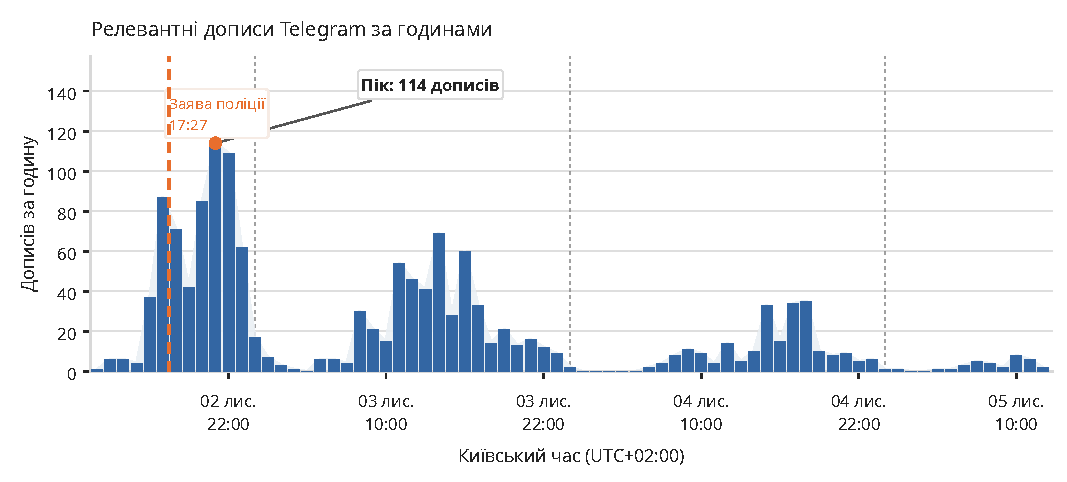
\includegraphics[width=\linewidth]{fig1_telegram_timeline_uk}
\caption{Погодинна кількість релевантних дописів у цільовій панелі Telegram, 2–5 листопада 2026 року.}
\label{fig:telegram-hourly}
\caption*{\small\textit{Примітка.} Десятихвилинні інтервали агреговано до годинних значень за київським часом (UTC+02:00; базовий набір $n=1{,}408$). Помаранчева позначка відповідає заяві Національної поліції о 17:27; часовий порядок не доводить впливу. Джерела: базовий часовий ряд і заява поліції \citep{socialreport2026,npu2026statement}.}
\end{figure}

\subsection{Твердження, наративи та невирішені фізичні факти}

Правиловий пошук знайшов 301 допис із згадкою заручників/незаконного утримання, 505 — смерті/катувань, 230 — фрази «концтабір ТЦК», 81 — приховування доказів, 307 — офіційної версії або спростування. Категорії перетинаються, а позиція автора не валідована, тож ці кількості не означають число людей, які повірили кожному твердженню. Найважливіший методологічний результат — не вердикт про поширеність наративів, а продемонстрований розрив між лексичним пошуком і встановленням позиції чи істинності.

На рис.~\ref{fig:narrative-mentions} наведено ці кількості правилового пошуку; категорії багатоміткові й дослідницькі.

\begin{figure}[!htbp]
\centering
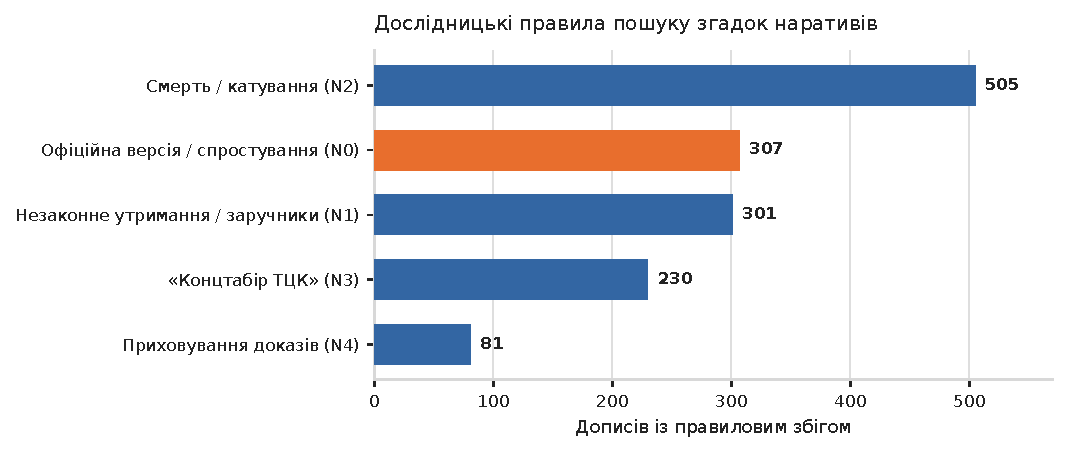
\includegraphics[width=\linewidth]{fig2_narrative_mentions_uk}
\caption{Дописи з принаймні одним правиловим збігом наративу в базовому корпусі.}
\label{fig:narrative-mentions}
\caption*{\small\textit{Примітка.} Категорії перетинаються: один допис може відповідати кільком правилам. Класифікатор недостатньо валідований для оцінювання поширеності чи позиції автора. Джерело: агрегація наративів базового набору \citep{socialreport2026}.}
\end{figure}

У 25-позиційній матриці доказів лишаються невстановленими два центральні фізичні твердження: що 40 цивільних незаконно утримували та що цивільна особа загинула. Поліція й Нацгвардія заперечували ці твердження; проєкт зберігає заперечення як позицію установ. Доступні матеріали не містять незалежного поіменного перепису або повної доказової бази, яка встановлювала б чи спростовувала обидва фізичні твердження. Це не підтримка жодної зі сторін. У публічних повідомленнях також ішлося про чотирьох травмованих військовослужбовців, які отримували медичну допомогу, однак проєкт не отримав медичних документів для незалежного встановлення характеру, часу й причин травм. Одне публічне повідомлення цитувало командира щодо раніше діагностованого перелому хребця після навчань в іншій частині; це не встановлює травму під час цього інциденту.

Процесуальні оновлення так само мають визначений обсяг. Якщо джерело підтверджує оголошення перевірки чи провадження, встановлення осіб, повідомлення про підозру або запобіжний захід, можна засвідчити відповідну процесуальну подію як повідомлену. Жодна з них не дорівнює встановленню вини. Презумпція невинуватості та неповнота відкритого провадження роблять персональні причинні наративи особливо недоречними.

Розподіл статусів усіх 25 оцінених тверджень із визначеним обсягом показано на рис.~\ref{fig:claim-status}.

\begin{figure}[!htbp]
\centering
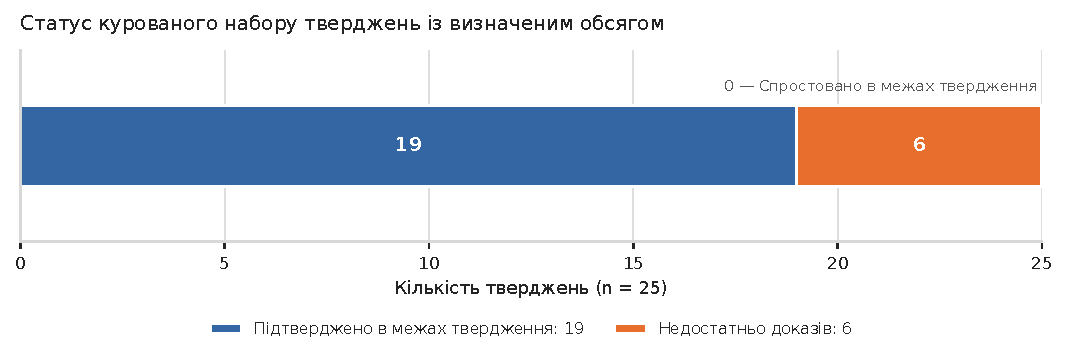
\includegraphics[width=\linewidth]{fig3_claim_status_uk}
\caption{Статуси 25 тверджень у курованому наборі з визначеним обсягом перевірки.}
\label{fig:claim-status}
\caption*{\small\textit{Примітка.} Статус «підтверджено в межах твердження» охоплює також висловлювання джерел і процесуальні події; він не означає незалежної перевірки 19 спірних фізичних тверджень. Матриця обмежена наданим корпусом і не є ані відкритим пошуком в інтернеті, ані судовим встановленням фактів. Джерело: запис верифікації тверджень \citep{socialclaims2026}.}
\end{figure}

\subsection{Поточні лічильники переглядів і невизначеність груп каналів}

У базовому наборі з 1\,408 дописів сума зафіксованих поточних лічильників переглядів становить 115\,931\,014. Це не унікальне охоплення: один користувач може переглядати допис повторно, аудиторії різних каналів перетинаються, лічильники не зафіксовано в момент публікації, а в 49 релевантних дописів лічильника не було. В окремому розширеному знімку з 1\,438 дописів сума поточних лічильників — 119\,515\,745. Різницю між сумами не можна трактувати як приріст унікальної аудиторії, оскільки відрізняються і вибірка, і час знімка.

Одна дослідницька перехресна таблиця показала, що 95,7\% поточної суми переглядів дописів із міткою N3 припадало на групу російських/проросійських каналів; після вилучення спірних та автоматичних міток частка становила 88,9\% у меншій підвибірці. Інтерпретація цього результату нестійка: мітки наративів не є валідованими позиціями, групи каналів поєднують різні виміри доказів, панель цільова, а перегляди сильно сконцентровані в кількох великих каналах. Ми не використовуємо результат для висновку про державну координацію чи переконання аудиторії. Це лише аналіз чутливості, який треба переоцінити після незалежного кодування каналів і наративів.

\subsection{Повторюваний текст і поведінкова координація}

Точний аудит графа виявив майже дубльовані дописи в багатьох каналах, а перестановочні тести показали, що деякі статистики часу й шаблонів нетипові для вибраних умовних моделей. Окремо ручний перегляд виявив кластер із 438 шаблонних коментарів від 367 псевдонімізованих акаунтів у чотирьох гілках Telegram. Строгіше кодування S7 і нульові моделі використовують інший словник фраз та інший знаменник; їх не слід об'єднувати, ніби це результат одного класифікатора.

Докази підтримують твердження, що копіювання й синхронізовані часові патерни були присутні, а деякі з них були концентрованішими за розподіл у заданих нульових моделях. Вони не встановлюють, що всі акаунти автоматизовані або оплачені, що один оператор віддавав накази, що їх контролювала організація чи що патерн змінив фізичний перебіг події. Платформна позначка бота була лише в невеликої кількості акаунтів; її немає підстав вважати повним детектором ботів. Ризики хибнопозитивної автоматичної класифікації ботів залежать від цільової групи та базової частки ботів \citep{rauchfleisch2020false}. Координація може виникнути внаслідок спільного інфоприводу, заклику до дії, норм спільноти або цілеспрямованої організації; подібність текстів не дозволяє розрізнити ці пояснення.

На рис.~\ref{fig:coordination-null} спостережену часову статистику порівняно з її умовним нульовим розподілом.

\begin{figure}[!htbp]
\centering
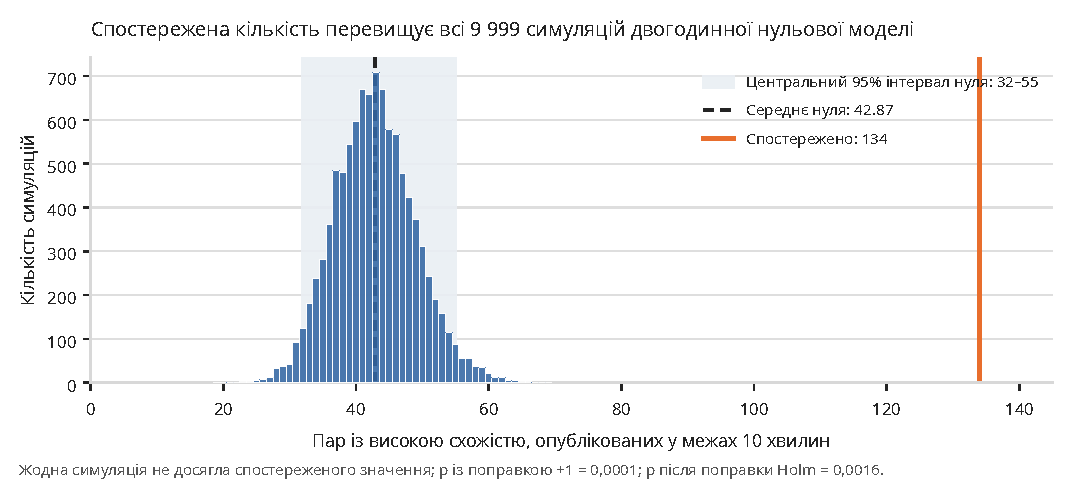
\includegraphics[width=\linewidth]{fig4_coordination_null_uk}
\caption{Спостережена кількість і нульовий розподіл пар високосхожих дописів, опублікованих із різницею до десяти хвилин.}
\label{fig:coordination-null}
\caption*{\small\textit{Примітка.} Статистика охоплює пари зі схожістю Жаккара $\geq 0{,}60$ серед 369 перевірених пар. Нульова модель — 9\,999 перестановок двогодинних часових слотів каналів; спостережено $=134$, середнє нуля $=42{,}87$, центральний 95\% інтервал $=32$–$55$, $p$ із поправкою +1 $=0{,}0001$, $p$ після поправки Holm $=0{,}0016$. Це дослідницький умовний тест, а не апостеріорна ймовірність маніпуляції чи державного керування. Джерело: результати перестановочного аналізу \citep{socialcoordination2026}.}
\end{figure}

\subsection{Окремий наратив про пожежу та невстановлене походження відео}

У знімку 883 коментарів TikTok 69 коментарів, відібраних правилами, переглянули вручну. Серед них 21 підтримував або натякав на версію «замітання слідів», а 20 виправляли географію. Решта переглянутих коментарів заперечували, ставили під сумнів або висміювали інтерпретацію, чи були неясними. Інші 814 коментарів вручну не кодували. Ці кількості документують різні інтерпретації у відібраній підвибірці, але не оцінюють їхню частку серед усіх коментарів і не встановлюють походження наративу.

Хронологія джерел відокремлює повідомлення про складську пожежу в Бучанському районі від місця попереднього зіткнення. Пізніший допис сільради назвав Софіївську Борщагівку, тоді як текст, накладений на відео, є лише підписом завантажувача. Перетин кадрів між файлами не встановлює місце сцени чи час зйомки. Наявні докази сумісні з географічною плутаниною, навмисним повторним використанням матеріалу або іншим поясненням, але не дозволяють вибрати між ними. Обережний висновок такий: коментарі показують спірну асоціацію з місцем, тоді як походження відео й шлях поширення не встановлено.

\subsection{Міжплатформне покриття і транскрипція мовлення}

42 посилання TikTok дали ідентифікатори коментарів і видимі лічильники, але вибірка задана користувачем, а фотоматеріали не завантажувалися. 9\,653 зібрані коментарі в цьому наборі посилань складаються з 3\,383 коментарів верхнього рівня та 6\,270 відповідей. Ідентифікатори коментарів верхнього рівня становили 28,17\% суми лічильників платформи за 41 елементом; це показник покриття відносно видимих лічильників, а не ймовірність включення. Для 32 із 41 елемента отримано менше ID, ніж показував лічильник. Відсутність коментаря про зв'язок пожежі із Софіївською у цьому обмеженому наборі не спростовує твердження в іншому відео чи на іншій платформі.

Корпус YouTube також сформовано за кандидатами. 444 лексичні збіги не є результатом перевірки повних відео. Фрагмент субтитрів може свідчити, що певні слова прозвучали або були процитовані, але без контексту не встановлює схвалення мовцем. Покриття Instagram, X, Threads і Facebook неповне або недоступне, тож відсутність записів трактується як відсутність доступу, а не як відсутність обговорення.

Високий загальний WER бенчмарку мовлення (44,58\%) і лише 10 безпечних для цитування кліпів із 18 підтримують обережну політику: автоматична транскрипція — інструмент індексації, а не дослівне першоджерело; цитати високої чутливості потребують прослуховування точного інтервалу або іншого незалежного еталона. Навіть виправлений транскрипт підтверджує лише слова, які чути у фрагменті; він не засвідчує особу мовця, істинність, правове значення чи описану подію.

На рис.~\ref{fig:asr-error} наведено макро- й мікроусереднені частки помилок слів у чотирьох цільово відібраних акустичних стратах.

\begin{figure}[!htbp]
\centering
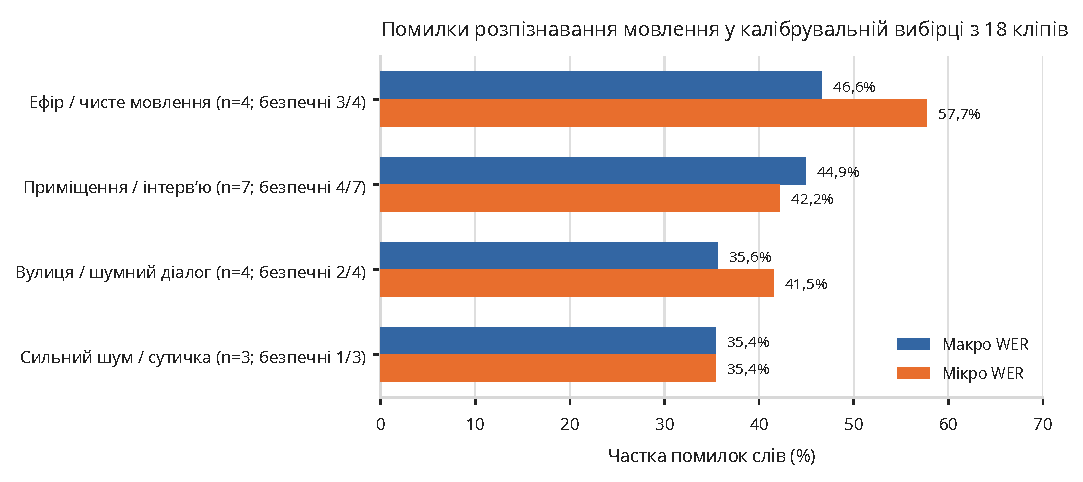
\includegraphics[width=\linewidth]{fig5_asr_error_uk}
\caption{Частки помилок розпізнавання мовлення у калібрувальній вибірці з 18 кліпів.}
\label{fig:asr-error}
\caption*{\small\textit{Примітка.} Стовпчики показують макро- та мікро-WER за цільово відібраними акустичними стратами; $n$ і кількість кліпів, безпечних для цитування, наведено біля назв страт. Перевірку цитат пройшли 10 із 18 кліпів. Результат не оцінює якість для всіх 607 архівованих файлів. Джерело: калібрувальний бенчмарк ASR \citep{socialasr2026}.}
\end{figure}

\section{Обговорення}

\subsection{Що підтримує цей кейс}

Зібрані матеріали підтверджують обмежений опис інформаційної хвилі в моніторингових каналах: високу кількість дописів 2–3 листопада, повторювані публічні твердження, подальші заяви установ і медіа, а також вимірювані патерни копіювання та синхронізації у вибраних записах Telegram. Вони також підтверджують наявність процесуального реагування, оскільки кілька установ публічно оголосили про перевірки та слідчі кроки. Пізніше обговорення пожежі містить виразну суперечку про географічну прив'язку у цільовій вибірці коментарів.

Дослідження не встановлює повної фізичної послідовності подій, істинності всіх тверджень про умови, джерела кожного наративу, кампанію під керуванням держави або вплив онлайн-контенту на учасників. Найсильніший висновок має методологічний характер: цифрові сліди дають змогу вимірювати записи й зберігати атрибутовані твердження, але не скасовують різниці між подією, повідомленням про подію та твердженням про повідомлення.

\subsection{Чому кількість джерел не дорівнює незалежності доказів}

Багато дописів можуть повторювати одне першоджерело. Якщо рахувати кожен репост як незалежне підтвердження, виникає хибна впевненість. У проєкті зафіксовано частину відомих залежностей між джерелами, але незалежність коренів походження не перевірялася зовнішньо. Подальші звіти мають розрізняти кількість публікацій і кількість незалежних першоджерел, показувати ланцюг залежності для повторюваних тверджень. Дизайн FEVER та AVeriTeC підкреслює користь пошуку й подання конкретних фрагментів доказів, але результати бенчмарків також демонструють складність отримання одночасно правильного вердикту й належних доказів \citep{thorne2018fever,schlichtkrull2023averitec,schlichtkrull2024averitecshared}. У цьому кейсі зовнішньо встановлена істина про фізичні обставини лежить поза доступною доказовою базою проєкту.

\subsection{Чому значущий координаційний тест не є атрибуцією}

Умовний перестановочний тест запитує, чи є підсумкова статистика нетиповою щодо певної рандомізації, яка зберігає вибрані властивості. Він не перевіряє пояснення, не включене в модель. Оскільки корпус цільовий, кандидатні кластери виявлялися під час дослідницького аналізу, а зіставного набору органічних подій немає, p-значення слід читати як умовний доказ проти конкретних нульових моделей, а не як апостеріорну ймовірність маніпуляції. Старберд та колеги описують дезінформаційну діяльність як колективну роботу за участю організованих акторів і звичайних користувачів; тому координація має спершу описувати спостережувану поведінку, а не командну структуру \citep{starbird2019collaborative}. Дослідження координованої поведінки також вимагають враховувати кілька поведінкових вимірів і рамку збору даних \citep{pacheco2021uncovering,nizzoli2021coordinated,magelinski2022synchronized,ng2023combined}.

\subsection{Цінність явного визнання невідомого}

Корисний звіт не зобов'язаний вирішувати кожне спірне питання. Він має показувати, які докази могли б змінити оцінку. У цьому кейсі це незалежні медичні документи, повний список осіб або журнал перебування, підписаний остаточний звіт перевірки, повні первинні медіафайли, аналіз геолокації TikTok-відео та архівовані матеріали найперших дописів. Матриця доказів уже розділяє твердження, підтримані в межах визначеного предмета, та твердження, для яких записів недостатньо. Такий підхід із відкритим світом знань не дозволяє перетворити відсутність оприлюдненого документа на доказ того, що подія не відбулася.

\section{Обмеження та дослідницька етика}

Панель каналів цільова й неповна; її результати не репрезентують Telegram і тим паче населення. Пошук і видимість можуть не охопити евфемізми, локальні алюзії, приватні групи чи інші мови. Час збору різниться між платформами, а видимі лічильники є знімками. Для базового корпусу з 1\,408 дописів і розширеного з 1\,438 різні межі збору; їх не слід об'єднувати без звірки на рівні записів.

Лексичний класифікатор наративів недостатньо валідований для кількох категорій. Другий LLM-анотатор не є незалежним людським еталоном; сама узгодженість не встановлює валідність конструкта. Координаційні тести використовують умовні нульові моделі, що можуть не відтворювати органічне копіювання після спільної новини; аналіз дослідницький, із поправкою Холма на 16 тестів, але не є підтверджувальним пререєстрованим експериментом. Вручну перевірена підвибірка коментарів TikTok мала й цільово відібрана. Поріг візуального збігу не калібрували. Вибірка транскрипції з 18 кліпів мала й не дає підстав переносити точність на всі 607 відео. Автоматизований рушій аналізу кейсу не оцінював семантичну точність, автентичність джерел, відповідність цитат доказам або істинність подій; набір структурних автоматичних перевірок не є семантичним еталоном \citep{socialcaseengine2026}.

Сирі дані містять коментарі користувачів і псевдонімізовані ідентифікатори. Псевдонімізація не гарантує анонімності, особливо коли текст можна знайти пошуком. Відповідно до етичних настанов для інтернет-досліджень, проєкт не публікує імена акаунтів, непотрібні персональні подробиці чи повні масиви сирих коментарів; подальше поширення потребує перевірки умов платформ, оцінки приватності й мінімізації пошукових цитат \citep{aoir2019ethics}. Внутрішні артефакти приватного репозиторію є аналітичним журналом проєкту, але не незалежним доказом і не відкритим пакетом відтворення.

\section{Висновки для систем аналізу інцидентів}

Цей кейс указує на багаторівневу архітектуру моніторингу, заснованого на доказах:
\begin{enumerate}
\item Спершу зберігати записи та їхнє походження, а вже потім інтерпретувати; окремо фіксувати час збору, публікації, події та оцінювання.
\item Представляти кожне положення як твердження, пов'язане з точним фрагментом джерела, походженням, типом зв'язку та статусом із визначеним обсягом.
\item Розрізняти тему згадки, позицію автора, позицію джерела й оцінку істинності. Збіг ключового слова є пошуковим сигналом, а не міткою переконання.
\item Вести окремо хронологію комунікації та фізичних подій. Об'єднувати згадки про події лише за наявності явних доказів і зберігати нерозв'язані альтернативи.
\item Використовувати точний аудит графів і аналіз чутливості для опису повторюваного тексту; позначати результат як поведінковий сигнал координації лише на рівні, який він підтверджує.
\item Трактувати перегляди, вподобання, відповіді й emoji як платформні сигнали залучення, а не як унікальне охоплення чи репрезентативне голосування.
\item Вимагати посилання на джерела для висновків згенерованого звіту й дозволяти системі відповідати «доказів недостатньо» або «визначити неможливо».
\end{enumerate}

Автоматизація найкраще підходить для детермінованих операцій: дедуплікації, нормалізації часу, хешування входів, квитанцій пошуку фрагментів, агрегування з фіксованими знаменниками та перевірок узгодженості звіту. Класифікація мови, незалежність джерел, сарказм, геолокація відео та причинна атрибуція потребують каліброваних моделей, належних доказів і явної невизначеності. Мета — автономна система, здатна утриматися від висновку, а не та, що заповнює кожне поле за будь-яку ціну.

\section{Висновок}

Кейс Петропавлівської Борщагівки показує і цінність, і епістемічні обмеження публічних цифрових слідів. У цільовій панелі Telegram інформаційна хвиля була сконцентрована в перші два дні, а деякі патерни повторів були синхронізованішими, ніж очікувалося за визначеними умовними нульовими моделями. Публічні заяви установ і повідомлення про розслідування можна відтворити як послідовність позицій джерел. Однак ключові фізичні твердження залишаються невирішеними в доступному корпусі, міжплатформні дані неповні, а конкретне відео пожежі незалежно не геолоковане.

Тому дослідження не проголошує остаточну фізичну версію подій, не називає прихованого організатора й не оцінює громадську думку. Воно документує, які твердження підтримуються спостережуваними записами, яким вони суперечать і чого дані не встановлюють. Для спірних подій ця межа не є недоліком, який треба приховати; вона сама є частиною результату. Звіт, який зберігає невизначеність, залежність джерел, знаменники й історію виправлень, корисніший за впевнену розповідь, побудовану на ототожненні повтору з підтвердженням або відсутності даних із доказом.

\section*{Заява про дані та матеріали}
На момент підготовки чернетки репозиторій Social є приватним. У статті наведено внутрішні артефакти проєкту й дати зрізів, але повний сирий корпус публічно не депоновано. Перед публічним випуском потрібен правомірний пакет відтворення, що захищає приватність, маніфест джерел із хешами та чіткий перелік недоступних чи обмежених матеріалів. Незалежного експертного визначення фізичних фактів для цього дослідження не було.

\section*{Конфлікт інтересів і фінансування}
Дослідження не отримувало зовнішнього фінансування. Автор заявляє про відсутність конфліктів інтересів.

\section*{Внесок автора та використання генеративного ШІ}
Олександр Пилипенко керував проєктом і визначав напрям дослідження та підготовки рукопису. Інструменти генеративного ШІ використовувалися для розроблення програмного забезпечення, підтримки обчислювального аналізу та підготовки тексту. Їхні результати не розглядаються як незалежні докази. Автор відповідає за остаточний перегляд, інтерпретацію та схвалення рукопису.

\section*{Подяки}
У проєкті використано відкриті заяви установ, доступні платформні записи та внутрішні матеріали збору й аудиту. Жодну особу не згадано на ім'я без її згоди.

\bibliographystyle{unsrtnat}
\bibliography{references}
\end{document}
